\documentclass[12pt, twoside]{article}
\usepackage[letterpaper, margin=1in, headsep=0.5in]{geometry}
\usepackage[english]{babel}
\usepackage[utf8]{inputenc}
\usepackage{amsmath}
\usepackage{amsfonts}
\usepackage{amssymb}
\usepackage{tikz}
\usepackage{venndiagram}


\usepackage{graphicx}
\usepackage{enumitem}
\usepackage{multicol}

\usepackage{fancyhdr}
\pagestyle{fancy}
\fancyhf{}
\renewcommand{\headrulewidth}{0pt} % disable the underline of the header

\fancyhead[RE]{\thepage}
\fancyhead[RO]{\thepage \\ Name: \hspace{3cm}}
\fancyhead[L]{BECA / Dr. Huson / 11.1 IB Math SL\\* 6 February 2018 \\* Classwork: Probability pretest practice \& review topics}

\begin{document}

\begin{enumerate}

\item For each Venn diagram, write an expression representing the shaded area.
\begin{enumerate}
    \item For example, for this diagram \\*
    %\\*
    \begin{venndiagram2sets}
        \fillANotB
        %\fillB
    \end{venndiagram2sets}
    Expression: $A \cap B'$\\*
    \item %\\*[15pt]
    \begin{venndiagram2sets}
        \fillNotB
    \end{venndiagram2sets}
    Expression: %\\*
    \item %\\*[15pt]
    \begin{venndiagram2sets}
    \fillBNotA
    \end{venndiagram2sets}
    Expression: %\\*
    \item %\*[15pt]
    \begin{venndiagram3sets}
    \fillB
    \fillCCapA
    \end{venndiagram3sets}
    Expression: %\\*
\end{enumerate}

\newpage
\item Given: \\*
\qquad $U = \{\text{the letters in the alphabet}\}$\\*
\qquad $A = \{a, b, c, d, e, f, g, h, i, j\}$
\qquad $B = \{h, i, j, k, l, m, n, o, p, q\}$
\begin{enumerate}
    \item What is $A \cap B$?\\*[20pt]
    \item What is $(A \cup B)'$?\\*[20pt]
\end{enumerate}

\item A survey question has three possible responses, $A$, $B$, and $C$. Among 100 surveys, the frequency of the answers collected were as follows: $n(A)=10, n(B)=35, \text{ and } n(C)=55$.
\begin{enumerate}
    \item If a survey is selected at random, what this the probability the response was $B$ or $C$?\\*[20pt]
    \item What is the probability a survey selected at random was an answer other than $B$ or $C$?\\*[20pt]
\end{enumerate}

\item The events $A$ and $B$ are independent with $\mathrm P(A)=0.3$ and $\mathrm P(B)=0.2$.
\begin{enumerate}
    \item What is $\mathrm P(A \cap B)$?\\*[20pt]
    \item What is $\mathrm P(A \cup B)$?\\*[20pt]
\end{enumerate}

\item The events $A$ and $B$ are mutually exclusive with $\mathrm P(A)=0.4$ and $\mathrm P(B)=0.3$.
\begin{enumerate}
    \item What is $\mathrm P(A \cap B)$?\\*[20pt]
    \item What is $\mathrm P(A^\prime \cup B)$?
\end{enumerate}


\newpage
\item The universal set $U$ is defined as the set of positive integers less than 15. The subsets $A$ and $B$ are defined as follows: \\*
\qquad $A =$ \{the even numbers\}\\*
\qquad $B =$ \{prime numbers\} \\* [5pt]
(note: Prime numbers have only themselves and one as factors. One is not considered a prime.)
\begin{enumerate}
    \item List the members of $A$\\*[20pt]
    \item List the members of $B$\\*[20pt]
    \item Place the elements of $A$ and $B$ in the appropriate regions in the Venn diagram below.\\*[5pt]
        \begin{venndiagram2sets}[tikzoptions={scale=2.5}]
        \end{venndiagram2sets}U\\*
    \item List the items in the set $(A \cup B)^\prime $\\*[20pt]
    \item If an element is selected at random, what is the probability that it is a member of the set $A \cap B$?
\end{enumerate}

\newpage
\item There are 90 juniors at a school taking courses as follows:
\begin{itemize}
  \item 27 are taking Algebra
  \item 35 are taking Botany
  \item 51 are taking Chemistry
  \item 11 are taking Algebra and Chemistry
  \item 6 are taking Algebra and Botany
  \item 13 are taking Botany and Chemistry
  \item 4 are taking all three subjects
\end{itemize}
Complete the Venn diagram below with the number of students in each region to represent the situation.
  \begin{center}
    \begin{venndiagram3sets}[tikzoptions={scale=2}]
    \end{venndiagram3sets}U
  \end{center}
How many juniors are taking none of the three courses?

\newpage
\item Let $y = x^2-5x+4$ and $2x+y=4$
\begin{enumerate}
    \item Rewrite quadratic in vertex form and state the vertex as an ordered pair.\\*[35pt]
    \item Factor the quadratic function and write down its roots.\\*[35pt]
    \item Graph the parabola, labeling it. Mark the intercepts and graph the axis of symmetry as a dotted line, labeling it with its equation.
    \item Graph linear equation and label it with its name or equation.
    \item Mark the intersections of the two equations as ordered pairs.

\end{enumerate}


\begin{figure}[!htbp]
\begin{center}
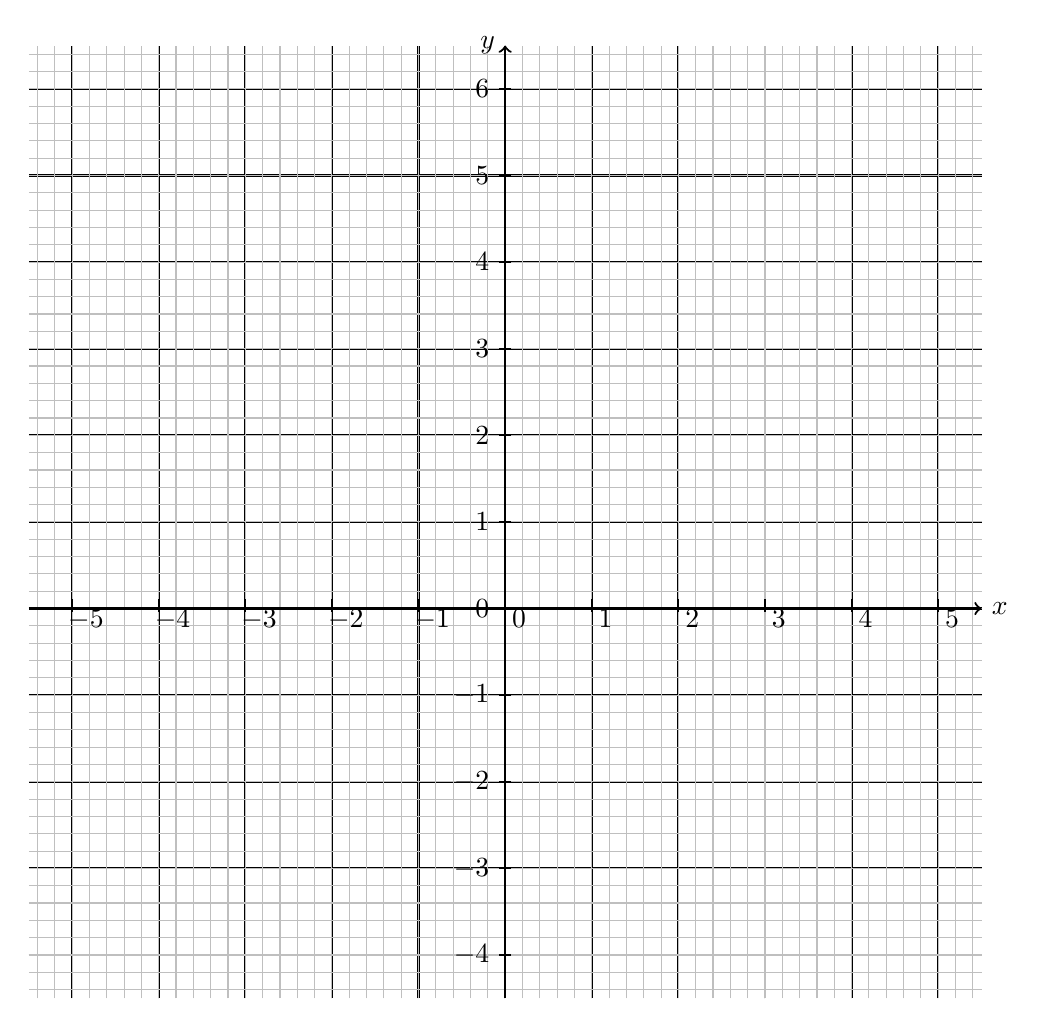
\begin{tikzpicture}[scale=1.1]

%grid
\draw [thick, color=black,, xstep=1.0cm,ystep=1.0cm] (-5.5,-4.5) grid (5.5,6.5);
\draw [thin, color=lightgray,, xstep=0.2cm,ystep=0.2cm] (-5.5,-4.5) grid (5.5,6.5);

\foreach \x in {-5, -4, -3, -2, -1, 0,1,2,3,4,5}
\draw[shift={(\x,0)},color=black] (0pt,-1pt) -- (0pt,3pt) node[below]  {$\quad \x$};

\foreach \y in {-4, -3, -2,-1,0,1,2,3,4, 5, 6}
\draw[shift={(0,\y)},color=black] (2pt,0pt) -- (-2pt,0pt) node[left]  {$\y$};

\draw [thick, ->] (-5.5,0) -- (+5.5,0) node [right] {$x$};
\draw [thick, ->] (0,-4.5) -- (0,6.5) node [left] {$y$};

%\draw [<-, ->] plot[domain= -3.5:2.5] (\x, \x*\x +\x -2);
%\draw [<-, ->] plot[domain= -5.5:3] (\x, \x+2);

\end{tikzpicture}
\end{center}
\end{figure}

\newpage
Simplify, leaving no negative or fractional exponents.

\item $2x^{-3}y \times \frac{1}{4}x^2 y^{-1}$\\*[45pt]
\item $\displaystyle a^{\frac{3}{4}} \times (\frac{\sqrt{a}}{b^4})^{\frac{1}{2}}$\\*[55pt]
\item $\ln{e^4}$\\*[35pt]
\item $\log 5^2 + \log 4$\\*[55pt]
\item $(2x^2-x-5)(x-3)-(x^2+3x-5)(2x-3)$\\*[85pt]
\item Factor the expression and then solve for $x$: $2x^3-2x^2-24x=0$

\newpage
\item Let $f(x) = 2x -5$ and $g(x)=(x-1)^2$
\begin{enumerate}
    \item Find $(f \circ g)(x)$\\*[65pt]
    \item Find $f^{-1}(x)$\\*[65pt]
\end{enumerate}

\item The function $f(x)=e^x$ is shown on the graph. Sketch $g(x)=f(x-2)+3$. Plot and label the asymptote(s).

\begin{figure}[!htbp]
\begin{center}
\begin{tikzpicture}

%grid
%\draw [thick, color=black,, xstep=1.0cm,ystep=1.0cm] (-5.5,-1.5) grid (5.5,16.5);
%\draw [thin, color=lightgray,, xstep=0.2cm,ystep=0.2cm] (-5.5,-1.5) grid (5.5,16.5);

\foreach \x in {-5, -4, -3, -2, -1, 0,1,2,3,4,5}
\draw[shift={(\x,0)},color=black] (0pt,-3pt) -- (0pt,3pt) node[below]  {$\x$};

\foreach \y in {-1,0,1,2,3,4,5, 6, 7}
\draw[shift={(0,\y)},color=black] (2pt,0pt) -- (-2pt,0pt) node[left]  {$\y$};

\draw [thick, ->] (-5.5,0) -- (+5.5,0) node [right] {$x$};
\draw [thick, ->] (0,-1.0) -- (0,7.5) node [left] {$y$};

\draw [<->] plot[domain= -3.5:2] (\x, e^\x);

\end{tikzpicture}
\end{center}
\end{figure}

\end{enumerate}

\end{document}


\item Using a calculator, find how many sets of three elements can be selected from a set of 8, when order does not matter, i.e. $_{8}\mathrm C_3$. \\*[20pt]
